

\documentclass[a4paper,12pt]{article}
\usepackage{amsfonts}
\usepackage{amsmath}
\usepackage{amssymb}
\usepackage{amsthm}
\usepackage{array}
\usepackage{fancyhdr}
\usepackage[colorlinks=true,allcolors=blue]{hyperref}
\usepackage[top=1in,bottom=2in,left=1in,right=1in]{geometry}
\usepackage{graphicx} \graphicspath{{figures/}}
\usepackage{subfigure}
\usepackage{color}
\usepackage[normalem]{ulem}

\usepackage{booktabs}
\usepackage{rotating,tabularx}


%\newcommand{\Mn}[1]{ \mathrm{M}_{#1}(\mathbb{R}) }
%\newcommand{\lex}{ \mathrm{lex} }
%\newcommand{\vect}{ \mathrm{vec} }
%\newcommand{\R}{\mathbb{R}}
%\newcommand{\x}{\mathbf{x}}
%\newcommand{\vv}{\mathbf{v}}
%\newcommand{\uu}{\mathbf{u}}
%\newcommand{\e}{\mathbf{e}}
%\newcommand{\rd}{\mathrm{d}}
%\newcommand{\re}{\mathrm{e}}
%\newcommand{\E}{\mathbb{E}}
%\newcommand{\Prob}{\mathbb{P}}
%\newcommand{\op}{\mathrm{op}}
\newtheorem{theorem}{Theorem}[section]
\newtheorem{lemma}[theorem]{Lemma}
\newtheorem{example}[theorem]{Example}
%\newtheorem{proposition}[theorem]{Proposition}
%\newtheorem{corollary}[theorem]{Corollary}
%\newtheorem{remark}[theorem]{Remark}
%\newtheorem{definition}[theorem]{Definition}
%\newtheorem{example}[theorem]{Example}

\newcommand{\diag}{\mathrm{diag}}
\newcommand{\tr}{\mathrm{tr}}




%\title{Free Music Archive (FMA): \\�A Dataset For Music Analysis}
\title{FMA: A Dataset For Music Analysis}


\author{Kirell Benzi, Micha\"el Defferrard, Pierre Vandergheynst, Xavier Bresson\\ \vspace{-0.5cm} \\  LTS2, EPFL, Lausanne, Switzerland}


\date{\today}




\begin{document}


%%%%%%%%%%%%%%%%%%%
\maketitle
%%%%%%%%%%%%%%%%%%%



%%%%%%%%%%%%%%%%%%%
\abstract{We present a new music dataset that can be used for several music analysis tasks. Our major goal is to go beyond the existing limitations of available music datasets, which are either the small size of datasets with raw audio tracks, the availability and legality of the music data, or the lack of meta-data for artists analysis or song ratings for recommender systems. Existing datasets such as GTZAN, TagATune, and Million Song suffer from the previous limitations. It is however essential to establish such benchmark datasets to advance the field of music analysis, like the ImageNet dataset which made possible the large success of deep learning techniques in computer vision. In this paper, we introduce the Free Music Archive (FMA) which contains 77,643 songs and 68 genres spanning 26.9 days of song listening and meta-data including artist name, song title, music genre, and track counts. For research purposes, we define two additional datasets from the original one: a small genre-balanced dataset of 4,000 song data and 10 genres compassing 33.3 hours of raw audio and a medium genre-unbalanced dataset of 14,511 data and 20 genres offering 5.1 days of track listening, both datasets come with meta-data and Echonest audio features. For all datasets, we provide a train-test splitting for future algorithms' comparisons. \\\\
{\it Keywords.} Music dataset, Free Music Archive (FMA), open science, reproducibility research, music analysis.} 
%%%%%%%%%%%%%%%%%%%





%%%%%%%%%%%%%%%%%%%
\section{Introduction and Motivation}
%%%%%%%%%%%%%%%%%%%

\noindent
{\bf Music Analysis Field.} Developing new mathematical models and algorithms to solve challenging real-world problems is obviously of first importance in any field of research. But such novel techniques must be evaluated and compared to the existing state-of-the-art techniques to be adopted as new standards by research communities. Evaluation and comparison require benchmark datasets to achieve their purpose, which are sometimes challenging to collect and share. In computer vision, the community has developed over the years well-established benchmark datasets such as MNIST \cite{pro:LeCunBottouBengioHaffner98MNIST} publicly accessible at \cite{art:MNIST}, CIFAR \cite{art:Krizhevsky09CIFAR} available at \cite{art:CIFAR}, or ImageNet \cite{art:FeiFei09ImageNet} provided at \cite{art:ImageNet}. All these image datasets are free, legal and easily available on Internet. Such datasets have proved essential to advance the field of computer vision. The most celebrated example is the ImageNet dataset and challenge in 2012. This unprecedented dataset of 1.5M image data allowed to demonstrate the power of deep learning techniques, which was able to win the competition by a large margin over the second best. In music analysis, such benchmark datasets are not easily available and they also lack of essential information. For examples, developing deep learning techniques for music applications require the use of raw audio data, and designing recommender systems need meta-data like artist features and song ratings. Besides, the most influential competition in the field of music analysis organized every year is the Music Information Retrieval Evaluation eXchange (MIREX) \cite{art:MIREX}. MIREX proposes several important music analysis challenges such as song identification, tag classification, music similarity and retrieval, etc. However, participants do not have access to neither the test set, nor the important train set. They must upload their code to a website that will be evaluated by the organizers. In other words, participants cannot train their analysis models on any part of the dataset. These existing shortcomings make essential the development of new music datasets to advance the field of music analysis.   \\


\noindent
{\bf Available music datasets and their limitations.} In music analysis, three datasets have been widely used by the international society for music information retrieval (ISMIR) \cite{art:ISMIR}: the GTZAN, TagATune, and MSD (Million Song Dataset) datasets. However each dataset come with some limitations: \\
$\bullet$ GTZAN \cite{art:TzanetakisCook02GTZAN} is a collection of 1000 songs with 10 music genres. Each song is represented by a 22,050Hz Mono 16-bit wav audio file of 30sec. It is the most popular music dataset with 6,600 answers on Google search, and 600 on Google scholar on Nov 2016. It has been widely used for different music applications. A complete study of this dataset was done in \cite{art:Sturm12GTZAN}, and the dataset is available at \cite{art:GTZAN}. The main limitations of GTZAN is the legality of the dataset, the small size, no complete meta-data regarding artist names and song titles, and no additional meta-data like ratings. \\
$\bullet$ TagATune \cite{art:Law07TagATune} was a popular dataset of 5,405 source songs of 230 artists. It was used for music tagging and music metric learning. Its website is \cite{art:TagATune}, but it is not anymore publicly available since 2009.\\
$\bullet$ The Million Song Dataset (MSD) \cite{art:Bertin11MSD} is a free and legal collection of 1 million music songs. Each song data is composed of high-level and medium-level audio features provided by  Echonest service and meta-data like artist name, song title, track genre, etc. It is available at \cite{art:MSD}. The very large scale of this music dataset would make it an ideal candidate for deep learning, which works best with large datasets. However, deep learning techniques work directly on the raw data (audio tracks in this case, like raw image pixels in computer vision) and not on pre-processed audio features given by Echonest. This prevents the application of deep learning on this dataset. Finally, Echonest reassigned the indexing of the MDS songs with its database, which henceworth makes (almost) impossible the use of the most music recent features developed by Echonest. \\


\newpage
\noindent
{\bf What would be the requirements for an ideal music dataset?}  \\
(1) Availability of raw audio tracks like 30sec or more,\\
(2) Availability of meta-data such as genres, artist, title, year, lyrics, users' ratings, users' comments, etc,\\
(3) Large-scale dataset to be able to sample the high-dimensional distribution of music genres\\
(4) Free and easy access of the dataset,\\
(5) Legality of the dataset, no copyright issue with e.g. open access licence.\\





%%%%%%%%%%%%%%%%%%%
\section{Introducing the FMA dataset}
%%%%%%%%%%%%%%%%%%%

\noindent
{\bf The website.} The FMA website \cite{art:FMA} is run by WFMU, the longest-running free-form radio station in the United States. The website provides a large catalogue of artists and high-quality mp3 songs. Each song is legally free to download as artists decided to work under open licence such as Creative Commons license. This is directly inspired by the open source movement, and the goal of the FMA site is to offer a legal and technological platform for artists and listeners to harness the full potential of online music sharing \cite{art:MossFMA}. FMA has been funded by the New York State Music Fund, the MacArthur Foundation, and the National Endowment for the Arts.\\



\noindent
{\bf Crawling the data.} The FMA organization provides an API \cite{art:FMA_API} to collect the meta-data associated to each song such as artist name, track title, track genre, and track listens. The collect of the mp3 audio files was done with a web scrapper. The collection of FMA was done in April 2016, and the size of the dataset at this time was 89,912 songs. It was recently announced on July 2016 that the website had reached the landmark of 100,000 songs. \\



\noindent
{\bf The raw FMA dataset.} The dataset collected on April 2016 contains 89,912 music data. As a first filtering, we kept the data that has audio tracks, reducing the size to 86,886 music data. All audio tracks are mp3-encoded with sampling rate of 44,100Hz, bit rate 128kb/s, and in stereo. Then, we considered the meta-data provided by the FMA website and crawled with its API. The meta-information collected is artist name, track title, track genres, and track listens. We removed data without genre information, giving 79,947 song data. Then, we created a top genre by simply picking the first genre in the original list of track genres provided by the artists. A few examples of data are given in Table \ref{tab1}. At this stage the number of genres is 138, but half have only a few samples. Thus we decided to only retain the genres with more than 100 samples. This defines a dataset of 77,643 music data with 68 genres. Figure \ref{fig_large} presents the distribution of the top 20 genres, which obeys to a power law distribution as often encountered in natural data collection. We further cleaned the dataset by removing tracks which belong to ``non-standard'' music genres like 'Noise', 'Garage', 'Sound Collage', 'Singer', 'Audio Collage', 'Glitch', 'Unclassifiable', 'Lo-Fi', 'Spoken', 'Poetry', 'Talk Radio', 'Avant-Garde', 'Experimental', 'Ambient', and 'Field Recording'. We also suppressed the songs with the title 'Untitled'. Besides, we decided to cut the long tail of the power law distribution by removing songs of genres with less than 300 songs. Finally, we kept the songs that have the raw audio and all Echonest features. Echonest features are medium-level and high-level audio features provided by Echonest \cite{art:Echonest}, a music platform for developers and media companies which has a collection of 3.5M artists and 37.5M songs. Echonest features can be either computed by uploading the songs to the Echonest website, which are then analyzed and send them back to the user, or simply retrieved from the Echonest database if the songs were analyzed before. All Echonest operations are done through an API \cite{art:Echonest_API}. Our final filtering consists in keeping songs that have both raw audio file and complete Echonest features already computed and stored in the Echonest database. The final size of the dataset is 14,511 music data and 20 genres. Figure \ref{fig_medium} presents the distribution of the genre sizes for this dataset. \\

  
 
\noindent
{\bf Proposed benchmark datasets.} For research purposes, we propose 3 datasets:\\
(1) FMA\_small: This dataset contains 4,000 songs with 10 genres equally balanced, that is 400 songs per class. For each song, we extracted 30sec precisely in the middle of the song. The total length is 33.3 hours of audio listening and the size is 3.4GB. The genre distribution is given in Figure \ref{fig_small}. The motivation for this dataset is to create an alternative to the popular GTZAN dataset with respect to the size and genre parameters. But unlike GTZAN, all songs have not only raw audio tracks but also meta-data composed of artist name, track title, track genres, track listens, and Echonest features. The GTZAN data may not have for example song title or artist name, and also no copyright permission. For reproducibility research, we also provide a train-test split 80-20 of this dataset for future techniques' comparisons.   \\
(2) FMA\_medium: This dataset has 20 genres with 14,511 songs of 30sec, also extracted from the middle of the track. The total length is 5.1 days of listening and the size is 12.2GB. Unlike FMA\_small, the size distribution of genres is not balanced, see Figure \ref{fig_medium}, but all songs have raw audio files and all meta-data i.e. artist name, track title, track genres, track listens, and Echonest features. We also provide a split 80-20 of this dataset.  \\
(3) FMA\_large: This dataset has 77,643 data of 30sec, again taken from the track middle, and 68 genres. It provides 26.9 days of track listening for 79.8GB. Figure \ref{fig_large} presents the top classes in the genre distribution. All songs come with the following meta-data: artist name, track title, track genres, track listens. Eventually, we give a split 80-20 of this dataset.\\


\noindent
Regarding the splitting train-test sets, we considered these constraints:\\
(a) For each genre, we randomly split train and test songs with the same ratio 80-20.\\
(b) We forced an artist to be either in the train set, or the test set (meaning the artist's songs cannot be in both train and test sets). \\
(c) We filled alternatively the train set and test set in the descending order of the count of artist songs. This prevented the test set to be filled with artists who have only a few songs.\\


\noindent
The FMA\_large dataset of 77,643 data contains songs of 30sec length, and artist name, track title, track genres, track listens as meta-data. Our original motivation was to give the full audio tracks, not limited to 30sec, but the size of the whole music tracks is 806.8GB (for approximatively 256 days of music listening) making the hosting a challenging issue.









%%%%%%%%%%%%%%%%%%%%
%\section{Classification Experiment [MICHAEL SECTION LATER LATER]}
%%%%%%%%%%%%%%%%%%%%
%
%\noindent
%{\bf Baseline classification techniques.}  In this section, we consider perhaps the most popular music analysis problem, the music genre recognition (MGR) problem. We apply standard baseline classification techniques on 2 representations of audio data: \\
%(1) Echonest medium-level 256-dim features, \\
%(2) Spectrograms of audio data by concatenating 10 spectrograms of 3sec into a single long vector.\\
%Table xxx reports the classification accuracy on the train and test datasets.\\
%
%
%\noindent
%{\bf Deep learning.} One major motivation to construct the FMA dataset was to apply the powerful deep learning techniques to the music analysis problem. As a preliminary result, we simply apply a convolutional neural network on the 3sec-spectrograms, and we select the class by majority voting. \\
%Table xxx reports the classification accuracy on the train and test datasets.\\


% TODO
% Problems
% Genre classif / mutli-genre classif
% Recommendation
% Play count prediction



%%%%%%%%%%%%%%%%%%%
\section{Conclusion and Perspectives}
%%%%%%%%%%%%%%%%%%%

\paragraph{Availability and reproducible research.}

All the datasets as well as Jupyter notebooks used to produce them, the
analysis, and baselines as are available online at

 \url{https://github.com/mdeff/fma}\\

 Code to support the use of the data is provided as well.
 
 
\paragraph{Potential applications.} We foresee multiple applications of this new dataset. The most obvious one is for music analysis with deep learning techniques. As raw music tracks are available, deep learning techniques like convolutional neural networks \cite{pro:LeCunBottouBengioHaffner98MNIST} and recurrent neural networks \cite{art:HochreiterSchmidhuber97LSTM} can be directly applied. Besides, standard data analysis tasks such as classification, clustering, regression, text analysis, visualization can also be applied to this new music dataset.\\



\section*{Acknowledgments}

We are grateful to SWITCH and EPFL for hosting the dataset within the context
of the \href{https://projects.switch.ch/scale-up/}{SCALE-UP} project, funded in
part by the swissuniversities \href{http://www.swissuniversities.ch/isci}{SUC
P-2 program}.




%%%%%%%%%%%%%%%%%%%
\vspace{1cm}
\bibliography{bib_paper}
\bibliographystyle{plain}
%%%%%%%%%%%%%%%%%%%

\newpage




\begin{figure}[h!]
\centering
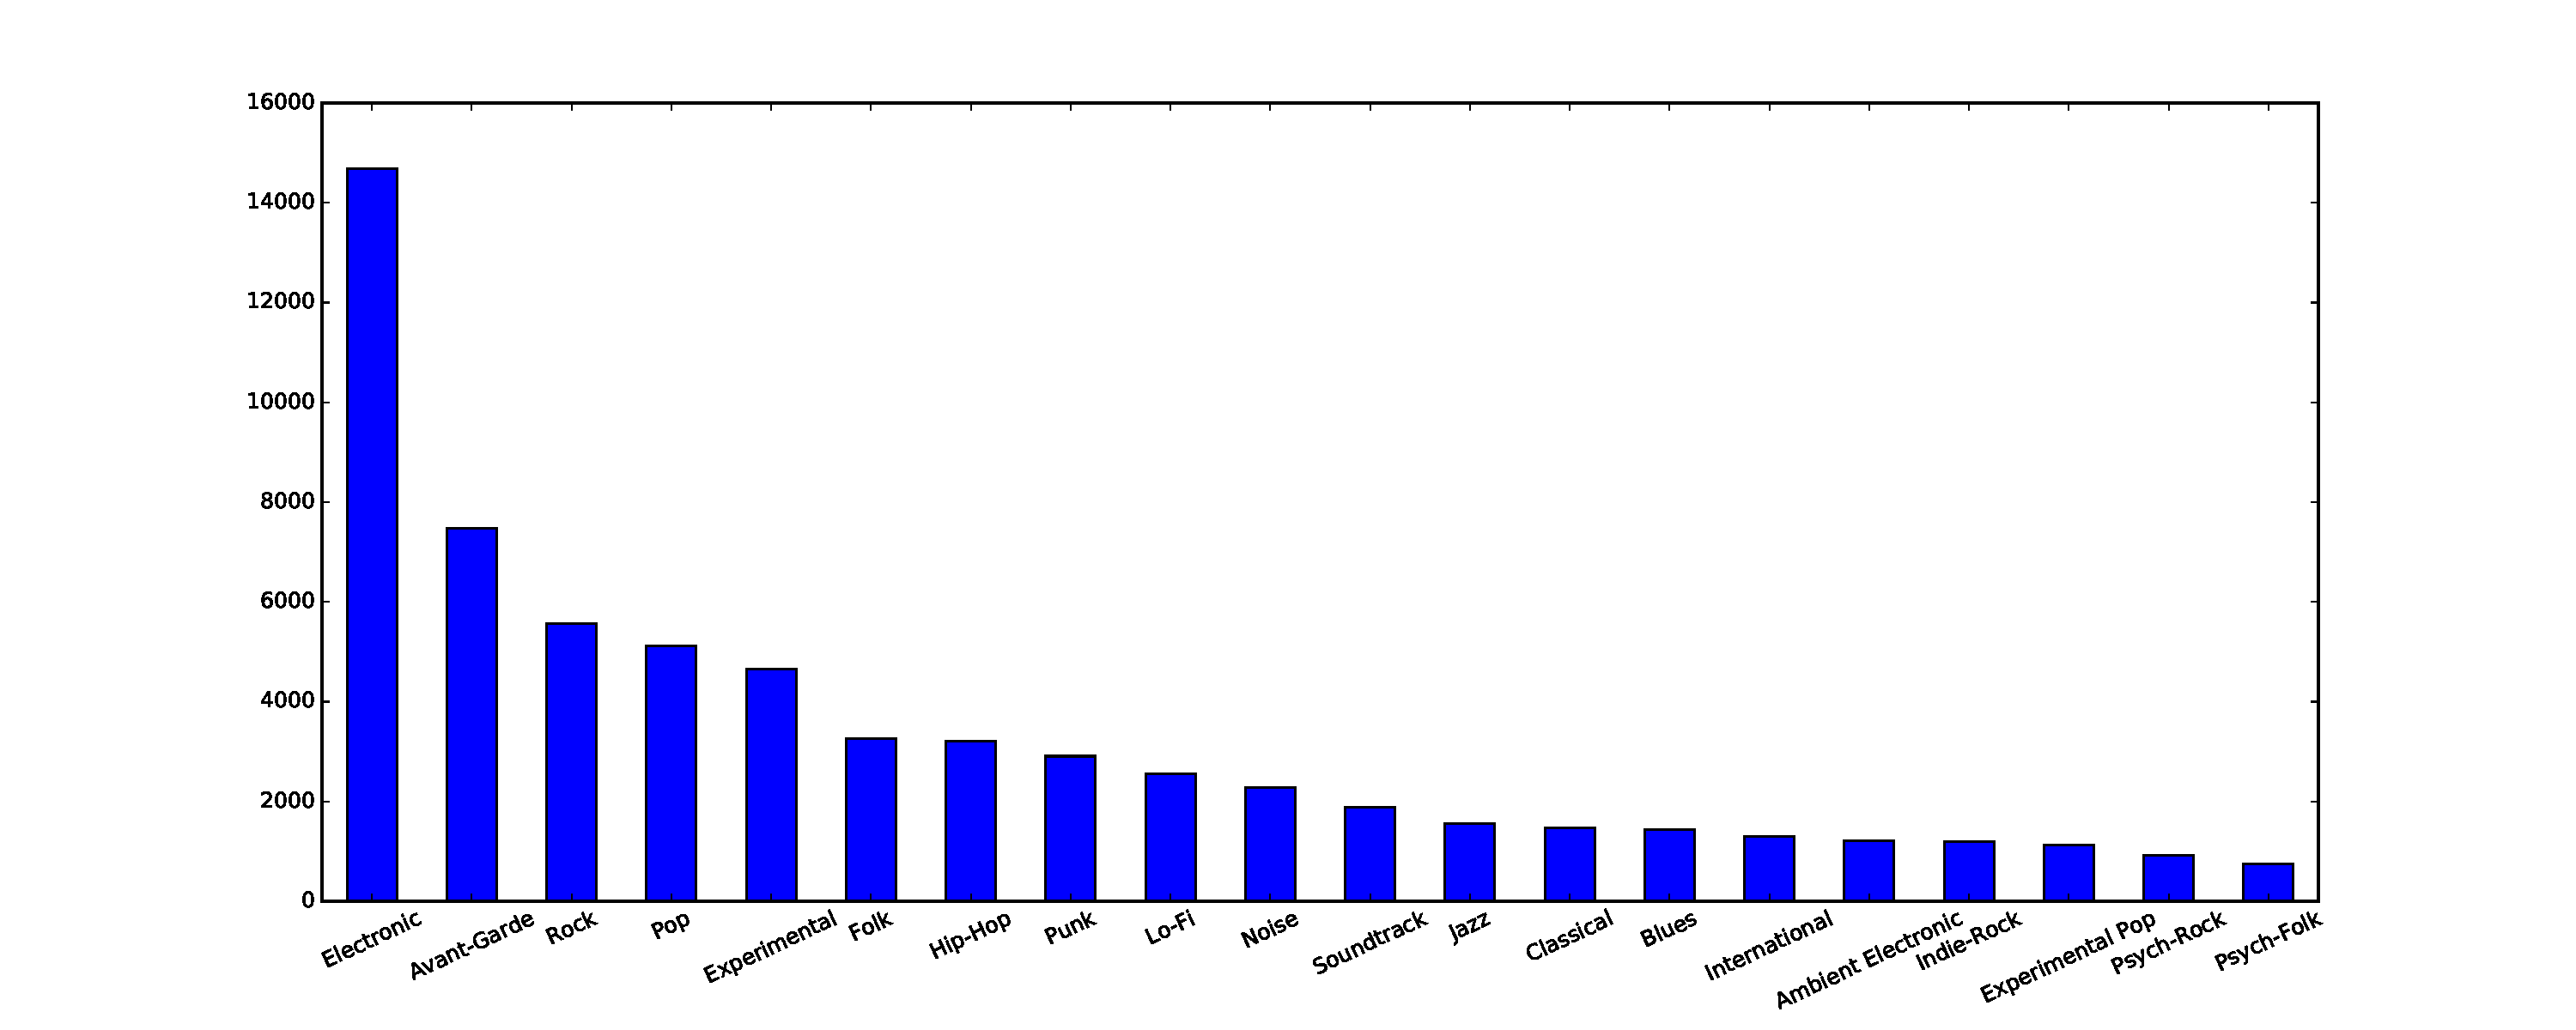
\includegraphics[height=6cm]{histo_large.pdf}
\vspace{-0.5cm}
\caption{Top 20 music genres for the FMA\_large dataset of 77,643 songs.}
\label{fig_large}
\end{figure}






\begin{figure}[h!]
\centering
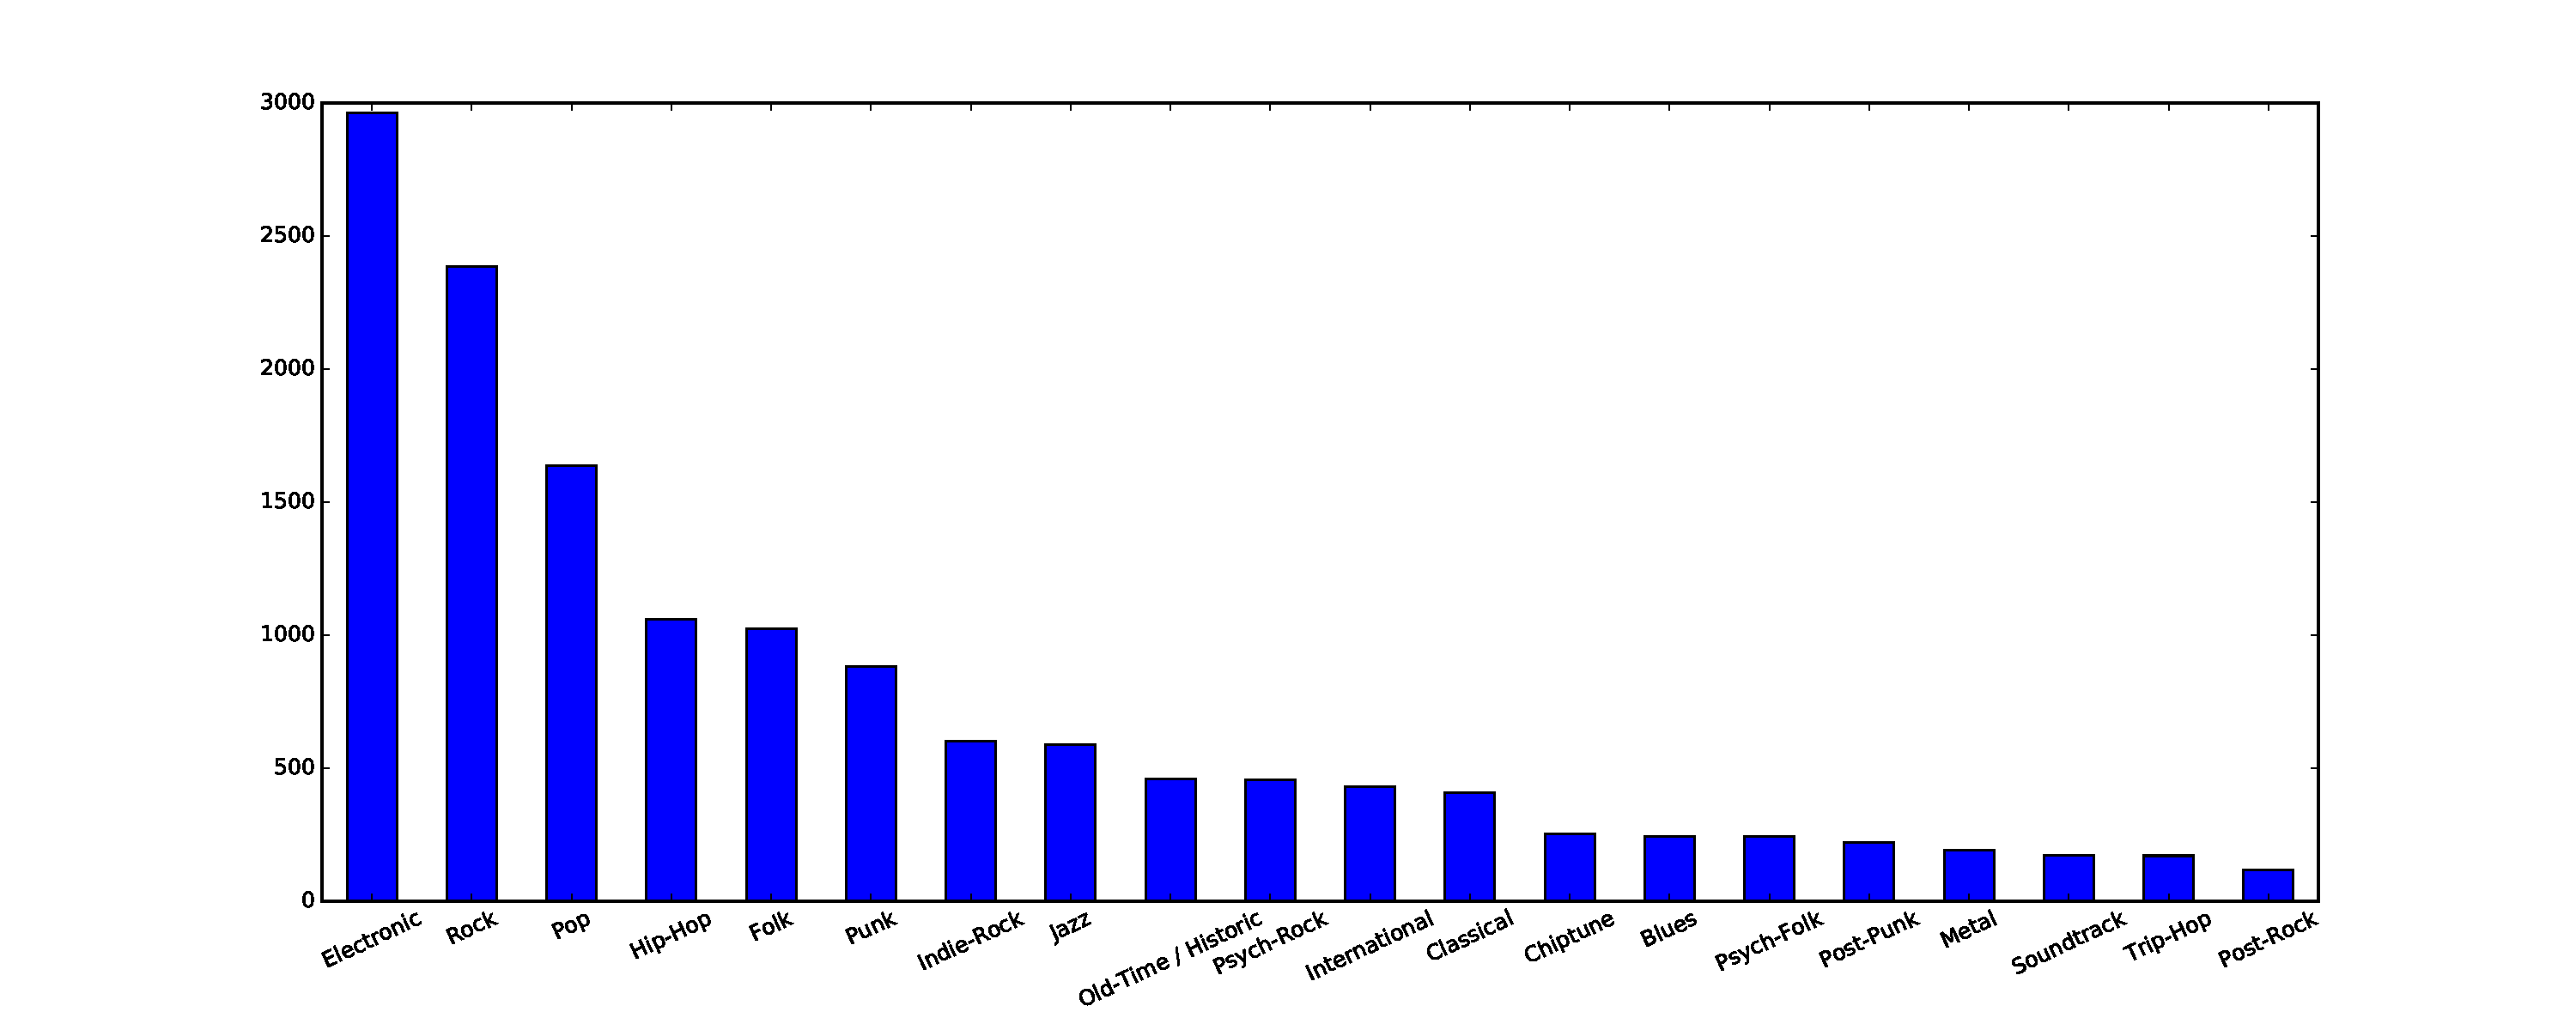
\includegraphics[height=6cm]{histo_medium.pdf}
\vspace{-0.5cm}
\caption{The 20 music genres for the FMA\_medium dataset with 14,511 songs.}
\label{fig_medium}
\end{figure}


\begin{figure}[h!]
\centering
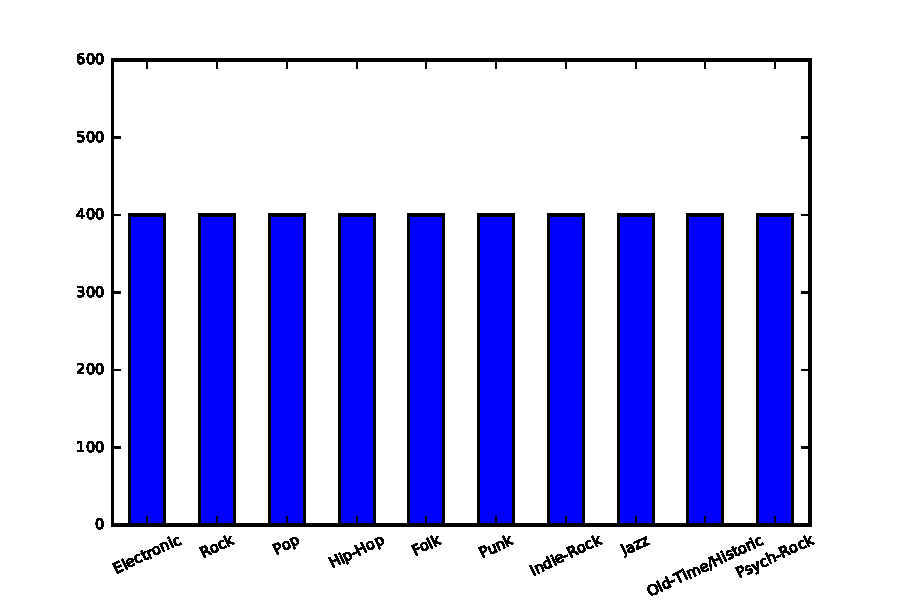
\includegraphics[height=5cm]{histo_small.pdf}
\vspace{-0.5cm}
\caption{The 10 music genres for the FMA\_small dataset with 4,000 songs.}
\label{fig_small}
\end{figure}


\newpage



%\begin{table}[h!]
\begin{sidewaystable}
\tiny{
\centering
\begin{tabular}{lrlrllll}
\toprule
 fma\_id &                                             artist &  play\_count &                                              title &                                             genres &            top\_genre  \\
 \toprule
    10 &                                          Kurt Vile &       42936 &                                            Freeway &                                              [Pop] &                  Pop  \\
    134 &                                               AWOL &         880 &                                       Street Music &                                          [Hip-Hop] &              Hip-Hop  \\
     141 &                    Alec K. Redfearn \& the Eyesores &         590 &                                               Ohio &                                             [Folk] &                 Folk  \\
     142 &                    Alec K. Redfearn \& the Eyesores &         670 &                               Punjabi Watery Grave &                                             [Folk] &                 Folk  \\
    144 &                                   Amoebic Ensemble &         901 &                                            Wire Up &                                             [Jazz] &                 Jazz  \\
   145 &                                   Amoebic Ensemble &         682 &                                         Amoebiasis &                                             [Jazz] &                 Jazz  \\
    188 &                                           Ed Askew &         973 &                                            Piano 1 &                                             [Folk] &                 Folk  \\
     206 &                                           Ed Askew &          73 &                                        Bella Crane &                                             [Folk] &                 Folk \\
     236 &                                       Banana Clipz &        6695 &                              Push Am (Left, Right) &                              [Electronic, African] &           Electronic  \\
     237 &                                          Barnacled &        1056 &                    Garbage and Fire &                                             [Jazz] &                 Jazz  \\
     238 &                                          Barnacled &         961 &                                     France Attacks &                                             [Jazz] &                 Jazz  \\
     461 &                              Cantonement Jazz Band &        3933 &                                           Bessemer &                               [Blues, Jazz: Vocal] &                Blues  \\
     462 &                              Cantonement Jazz Band &        3256 &                                     Has Been Blues &                               [Blues, Jazz: Vocal] &                Blues  \\
     463 &                              Cantonement Jazz Band &        3238 &                                       I'll Be Blue &                               [Blues, Jazz: Vocal] &                Blues  \\
    824 &                     Here Comes A Big Black Cloud!! &         391 &                                         Black Mold &          [Rock, Loud-Rock, Psych-Rock, Indie-Rock] &                 Rock  \\
     825 &                     Here Comes A Big Black Cloud!! &        1847 &                                        Death March &          [Rock, Loud-Rock, Psych-Rock, Indie-Rock] &                 Rock  \\
    837 &                                          Heroin UK &         146 &                                           DopeSick &                                             [Rock] &                 Rock \\
     889 &                                 Illusion of Safety &         163 &                                          Wasteland &                                       [Electronic] &           Electronic  \\
     896 &                                        Impediments &        1542 &                                               2012 &                                  [Punk, Power-Pop] &                 Punk  \\
          992 &                                      Jason Willett &         560 &                   Beautiful Song w/ kick drum solo &                                             [Rock] &                 Rock  \\
\bottomrule
\end{tabular}
\caption{A few song data in the FMA dataset.}
\label{tab1}
%\end{table}
}
\end{sidewaystable}






\end{document}





















